\documentclass[11pt]{article}
\usepackage{csc512}

%%% For FAS
\usepackage{tikz}
\usetikzlibrary{automata, positioning, arrows}

%%%%%%%%%%%%%%%%%%%% name/id
\rfoot{\small Brian Park | 200190057}


%%%%%%%%%%%%%%%%%%%% Course/HW info
\newcommand*{\instr}{Xu Liu}
\newcommand*{\term}{Fall 2022}
\newcommand*{\coursenum}{CSC 512}
\newcommand*{\coursename}{Compiler Construction}
\newcommand*{\hwnum}{1}

\rhead{\LARGE   \fontfamily{lmdh}\selectfont	HW \hwnum}

\lfoot{\small \coursenum, \term, HW \hwnum}

%%%%%%%%%%%%%%%%%%%%%%%%%%%%%% Document Start %%%%%%%%%%%%%%%%%
\begin{document}

%%%%%%%%%%%%%%%%%%%%%%%%%%%%%%%%%%%%%%%%%%%%%%%%%%%%%%%%%%%%%%%%%%%%%%%%%%%%%%%%%%%%%%%%
% Question 1
%%%%%%%%%%%%%%%%%%%%%%%%%%%%%%%%%%%%%%%%%%%%%%%%%%%%%%%%%%%%%%%%%%%%%%%%%%%%%%%%%%%%%%%%
\section*{1}
Describe informally the languages accepted by the following \verb|FAS|:

b.
\begin{Answer}
It only has one end state. It represents any pattern of \verb|1|s or \verb|0|s, but doesn't have a pattern for \verb|10| or \verb|01| after $s_1$ and $s_2$ which will be followed by a sequence of \verb|00| and \verb|11| respectively.
\end{Answer}

c.
\begin{Answer}
Will contain a lot of \verb|a|'s and \verb|b|'s. Subset of \verb|aab| and \verb|baa| will appear.
\end{Answer}

\newpage

%%%%%%%%%%%%%%%%%%%%%%%%%%%%%%%%%%%%%%%%%%%%%%%%%%%%%%%%%%%%%%%%%%%%%%%%%%%%%%%%%%%%%%%%
% Question 2
%%%%%%%%%%%%%%%%%%%%%%%%%%%%%%%%%%%%%%%%%%%%%%%%%%%%%%%%%%%%%%%%%%%%%%%%%%%%%%%%%%%%%%%%
\section*{2}
Construct an \verb|FA| accepting each of the following languages: \\

b. $w \in \{0, 1\}^* | w$ contains `111' as a substring and does not contain `00' as a substring

\begin{Answer}
\centerline{
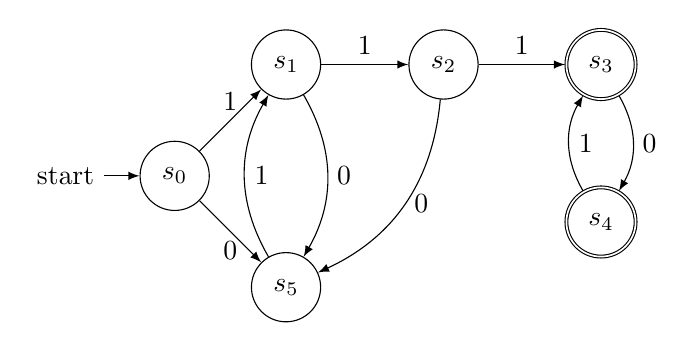
\begin{tikzpicture}[node distance = 2cm, on grid, >=latex]
    \node[state, initial] (0) {$s_0$};
    \node[state, above right of=0] (1) {$s_1$};
    \node[state, right of=1] (2) {$s_2$};
    \node[state, right of=2, accepting] (3) {$s_3$};
    \node[state, below of=3, accepting] (4) {$s_4$};
    \node[state, below right of=0] (5) {$s_5$};
	
	\draw[->] (0) edge[above] node{$1$} (1)
	(1) edge[below, bend left, right=0.3] node{$0$} (5)
	(5) edge[below, bend left, right=0.3] node{$1$} (1)
	(0) edge[below] node{$0$} (5)
	(1) edge[above] node{$1$} (2)
	(2) edge[below, bend left, right=0.3] node{$0$} (5)
	(2) edge[above] node{$1$} (3)
	(3) edge[below, bend left, right=0.3] node{$0$} (4)
	(4) edge[below, bend left, right=0.3] node{$1$} (3);
\end{tikzpicture}
}
\end{Answer}

c. $w \in \{a, b, c\}^* | \in w$ the number of $a$'s modulo 2 is equal to the number of $b$'s modulo 3
\begin{Answer}
\centerline{
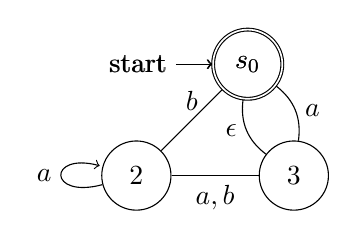
\begin{tikzpicture}[node distance = 2cm, on grid]
\node[state, initial] (1) {$s_0$};
\node[state, initial, accepting] (1) {$s_0$};

\node[state, below left of=1] (2) {$2$};
\node[state, right of=2] (3) {$3$};
\draw (1) edge[above] node{$b$} (2)
(1) edge[below, bend right, left=0.3] node{$\epsilon$} (3)
(2) edge[loop left] node{$a$} (2)
(2) edge[below] node{$a, b$} (3)
(3) edge[above, bend right, right=0.3] node{$a$} (1);
\end{tikzpicture}
}
\end{Answer}
\newpage

%%%%%%%%%%%%%%%%%%%%%%%%%%%%%%%%%%%%%%%%%%%%%%%%%%%%%%%%%%%%%%%%%%%%%%%%%%%%%%%%%%%%%%%%
% Question 4
%%%%%%%%%%%%%%%%%%%%%%%%%%%%%%%%%%%%%%%%%%%%%%%%%%%%%%%%%%%%%%%%%%%%%%%%%%%%%%%%%%%%%%%%
\section*{4}
Different programming languages use different notations to represent integers. Construct a regular expression for each one of the following: \\

c. Currency, in dollars, represented as a positive decimal number rounded to the nearest one-hundredth. Such numbers begin with the character \$, have commas separating each group of three digits to the left of the decimal point, and end with two digits to the right of the decimal point, for example, \$8,937.43 and \$7,777,777.77.

\begin{Answer}
$$\$\Big([1\cdots9]([0\cdots9] | \epsilon)([0\cdots9] | \epsilon)(,[0\cdots9][0\cdots9][0\cdots9])^*\Big|0\Big).[0\cdots9][0\cdots9]$$
\end{Answer}

\newpage

%%%%%%%%%%%%%%%%%%%%%%%%%%%%%%%%%%%%%%%%%%%%%%%%%%%%%%%%%%%%%%%%%%%%%%%%%%%%%%%%%%%%%%%%
% Question 5
%%%%%%%%%%%%%%%%%%%%%%%%%%%%%%%%%%%%%%%%%%%%%%%%%%%%%%%%%%%%%%%%%%%%%%%%%%%%%%%%%%%%%%%%
\section*{5}
Write a regular expression for each of the following languages: \\ 

e. Given an alphabet $\Sigma = \{+, -, \times, \div, (,), \verb|id|\}$, $L$ is the set of algebraic expressions using addition, subtraction, multiplication, division, and parentheses over \verb|id|s.

\begin{Answer}
$$L = \verb|id|\Big((+ | - | \times | \div)\verb|id|\Big)^+$$

An exception is that parenthesis cannot be matched with regular expression.
\end{Answer}

\newpage

%%%%%%%%%%%%%%%%%%%%%%%%%%%%%%%%%%%%%%%%%%%%%%%%%%%%%%%%%%%%%%%%%%%%%%%%%%%%%%%%%%%%%%%%
% Question 7
%%%%%%%%%%%%%%%%%%%%%%%%%%%%%%%%%%%%%%%%%%%%%%%%%%%%%%%%%%%%%%%%%%%%%%%%%%%%%%%%%%%%%%%%
\section*{7}
Consider the three regular expressions:
$$(ab | ac)^*$$
$$(0 | 1)^* 1100 1^*$$
$$(01 | 10 | 00)^* 11$$

a. Use Thompson's construction to construct an NFA for each RE. 

\begin{Answer}
\end{Answer}

b. Convert the NFAS to DEAS.

\begin{Answer}
\end{Answer}

c. Minimize the DFAs.

\begin{Answer}
\end{Answer}

\end{document}